\documentclass{article}
\usepackage[a4paper, margin=1in]{geometry}
\usepackage{amsmath}
\usepackage{graphicx}

\title{\textbf{Paper Review}}
\author{}
\date{}

\begin{document}

\maketitle

\section*{Title of the Paper:}
Training Compute-Optimal Large Language Models

\section*{Authors:}
[Insert Authors Here]
\section{Summary of the Paper}

\subsection{Research Objective}
The paper investigates the optimal trade-off between model size and number of training tokens for large language models (LLMs) given a fixed compute budget. The authors challenge the previous trend in the field where models are scaled primarily by increasing parameter count while keeping training data relatively constant.

\subsection{Key Contributions}
The paper makes several significant contributions to our understanding of LLM scaling laws. First, it demonstrates that current large language models are significantly undertrained and overparameterized relative to their compute budgets. Second, it establishes through multiple methodologies that model size (N) and training tokens (D) should scale equally with compute (C), contradicting previous scaling laws that favored increasing parameters over data. Finally, it validates these findings by introducing Chinchilla, a 70B parameter model that outperforms larger models like Gopher (280B) while using the same compute budget but training on more data.

\subsection{Methodology}
The authors present three complementary approaches to determine optimal scaling relationships. 
\subsubsection{Approach 1}
The first approach involves training multiple models of varying sizes (from 70M to 10B parameters) and training each model on four different amounts of data. The authors align learning rate schedules with training duration to ensure accurate and fair comparisons across different runs. This approach allows them to estimate the minimum achievable loss for each combination of model size, training duration, and data amount. By fitting a power-law model to the resulting data, they derive optimal scaling relationships between model size, training tokens, and compute, which helps guide efficient training strategies.
\begin{figure}[h]
    \centering
    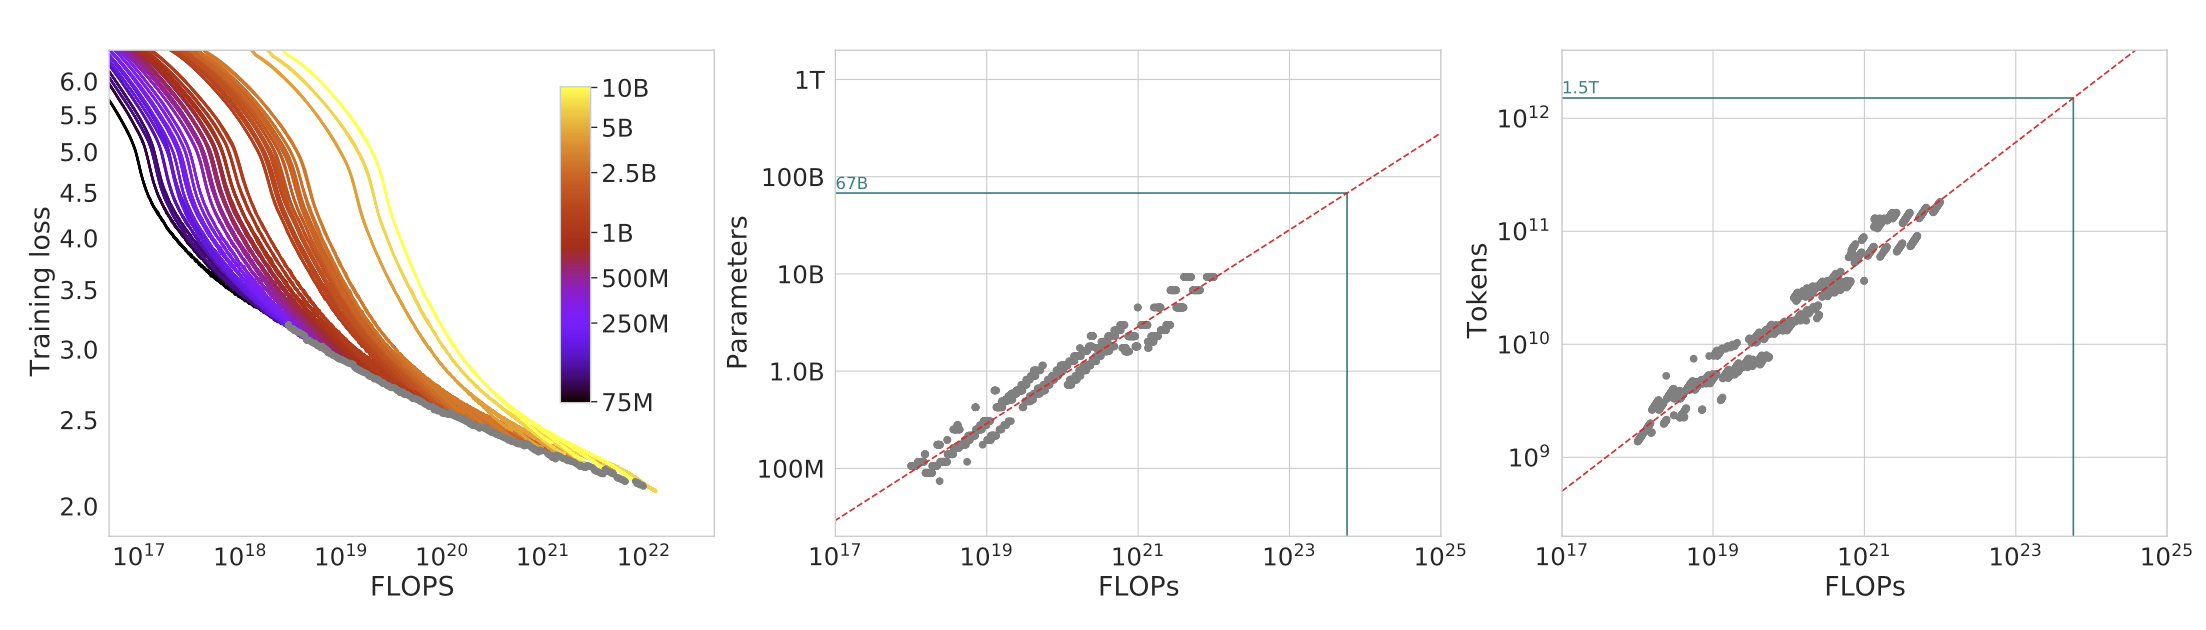
\includegraphics[width=0.9\textwidth]{figs/Approach1.png}
    \caption{Training curves for models ranging from 70M to 10B parameters, trained for four different durations.}
    \label{fig:approach1}
\end{figure}
\subsubsection{Approach 2}
The second approach involves setting nine different FLOP budgets, ranging from $6 \times 10^{18}$ to $3 \times 10^{21}$ FLOPs, and varying model sizes up to 16B parameters to analyze the final training loss at each budget. This method, known as IsoFLOP profiling, helps to answer the question: What is the optimal parameter count for a given FLOP budget? To ensure a clear minimum in loss, they trained a diverse set of model sizes, capturing comprehensive data across different scales. For each IsoFLOP profile, they fitted a parabolic curve to determine the optimal model size for each FLOP budget. Then, as in the previous approach, they fitted a power-law model to the data to identify optimal scaling relationship.
\begin{figure}[h]
    \centering
    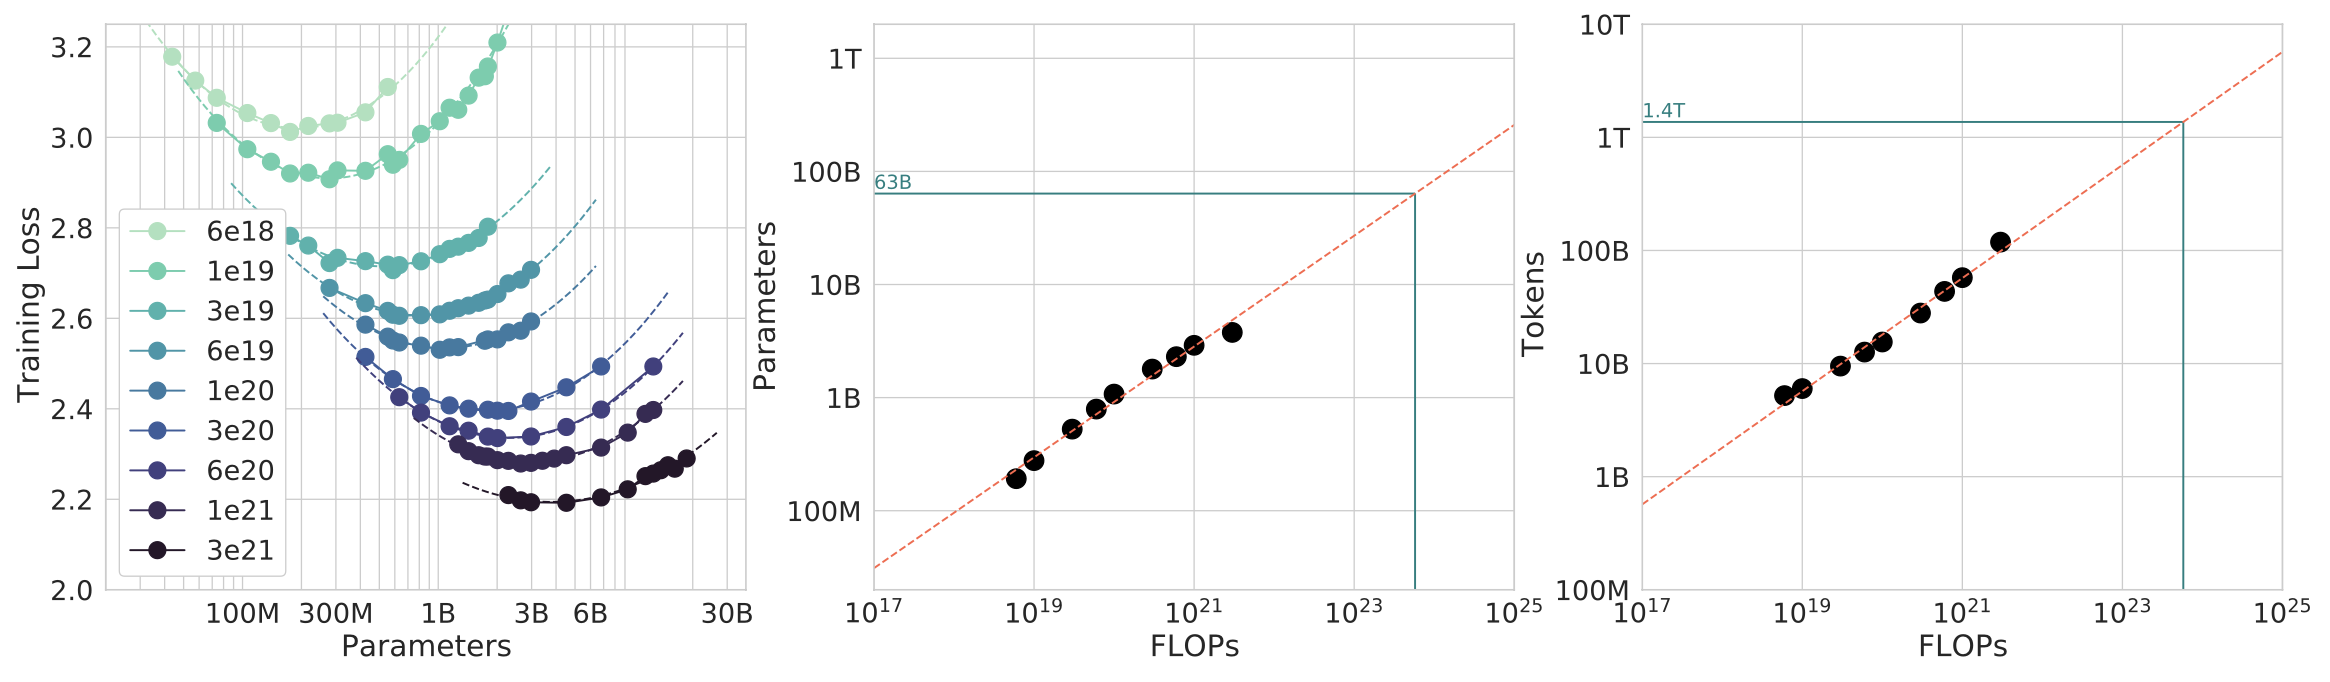
\includegraphics[width=0.9\textwidth]{figs/Approach2.png}
    \caption{IsoFLOP profiles for models ranging from 70M to 16B parameters, trained with nine different FLOP budgets.}
    \label{fig:approach2}
\end{figure}


\subsubsection{Approach 3}

The third approach proposes modeling loss as a function of parameter size and the number of tokens. Drawing from classical risk decomposition, this model defines loss as:


$$\hat{L}(N, D) = E + \frac{A}{N^\alpha} + \frac{B}{D^\beta}$$

$E$  represents the loss for an ideal generative process over the data distribution, which ideally aligns with the entropy of natural language. The second term,  $\frac{A}{N^\alpha}$ , acknowledges that even a perfectly trained transformer with  N  parameters falls short of the ideal generative process. Finally, the third term,  $\frac{B}{D^\beta}$ , captures the impact of not training the transformer to full convergence, due to limited optimization steps on a subset of the dataset.
To estimate the parameters  $A$ ,  $B$ ,  $\alpha$ , and  $\beta$ , the authors use a Huber loss function, which is robust to outliers, with  $\delta = 10^{-3}$ and applied the L-BFGS algorithm. The fitting process also involved a grid of initializations to avoid local minima.
For evaluating efficiency, the team used the parametric loss model to outline an efficient frontier of model performance under computational constraints. They identified optimal model and data parameters,  $N_{\text{opt}}$  and $ D_{\text{opt}}$ , by minimizing  $\hat{L}$  while adhering to the constraint  $\text{FLOPs}(N, D) \approx 6ND$ . This analysis provided a power-law relationship for  $N_{\text{opt}}$  and  $D_{\text{opt}}$ , balancing model size and data volume in a way that optimally manages computational resources.


\begin{figure}[h]
    \centering
    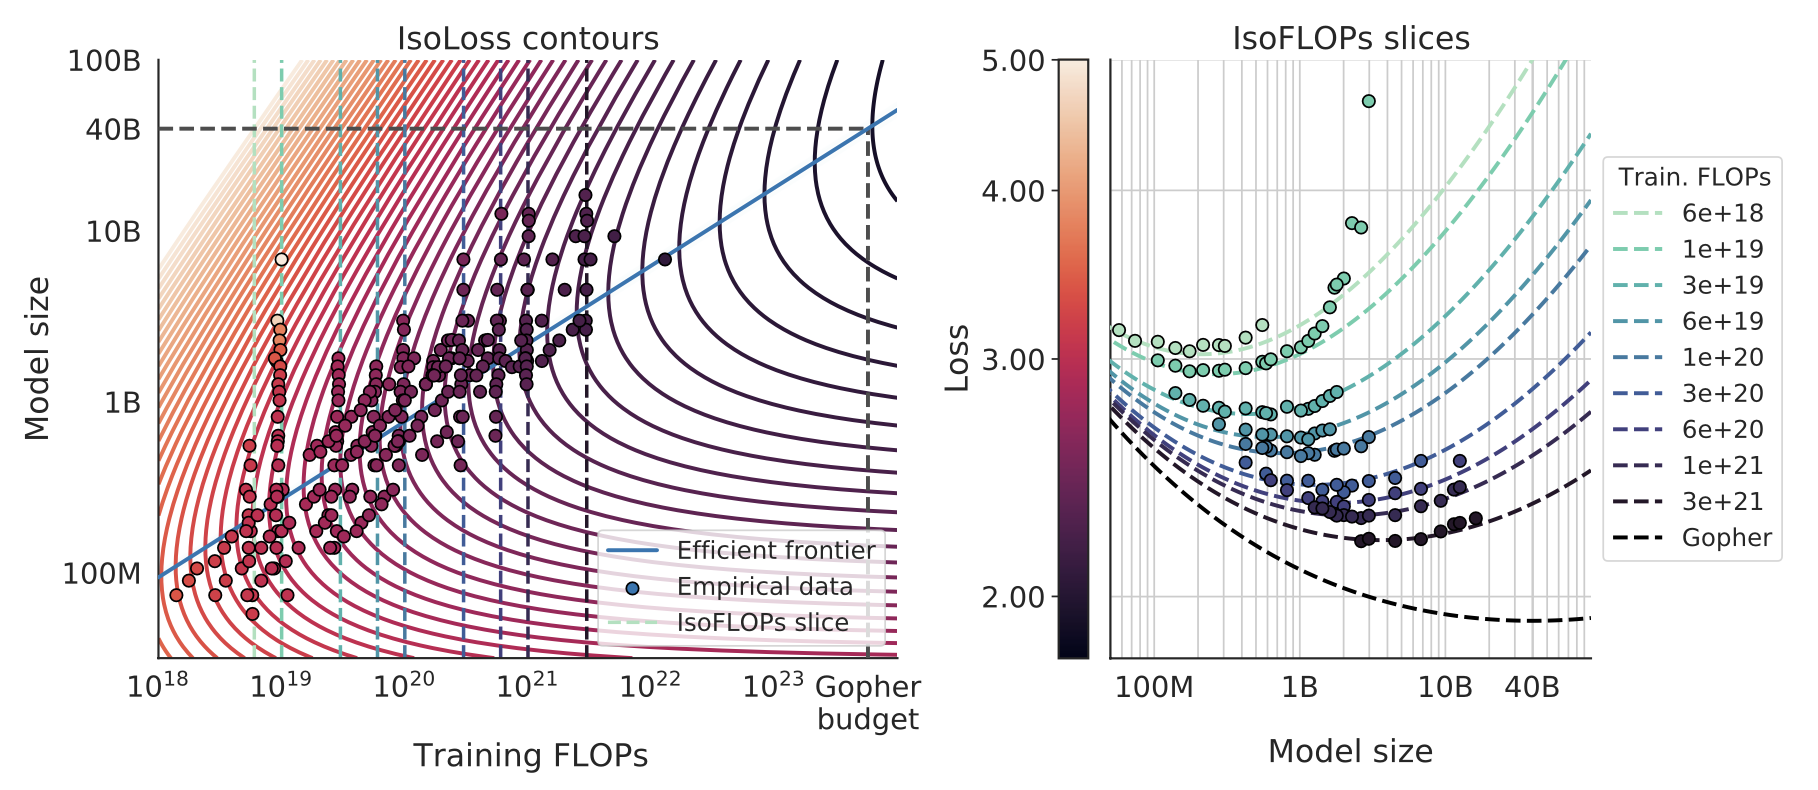
\includegraphics[width=0.9\textwidth]{figs/Approach3.png}
    \caption{Parametric loss model fitting for various model sizes and data amounts.}
    \label{fig:approach3}
\end{figure}


\subsection{Results and Findings}
All three methodological approaches converged on similar scaling coefficients, finding that optimal model size and training tokens should scale approximately as the square root of compute ($N_{opt} \propto C^{0.5}$, $D_{opt} \propto C^{0.5}$). This finding was validated through the training of Chinchilla, a 70B parameter model trained on 1.4T tokens, which consistently outperformed Gopher (280B parameters, 300B tokens) across most benchmarks despite using the same compute budget. These results strongly suggest that current large models are significantly oversized for their compute budgets and would benefit from being smaller but trained on more data.

\section{Critical Evaluation}

\subsection{Strengths}
The paper's primary strength lies in its methodological rigor and comprehensive empirical validation. The authors employ three distinct approaches to investigate scaling laws, each providing independent validation of their findings. This triangulation of methods significantly strengthens their conclusions. The identification and correction of the learning rate scheduling issue from previous work (Kaplan et al.) represents a crucial methodological improvement. By matching learning rate schedules to training duration, they obtain more accurate estimates of model performance with different amounts of training data.

The experimental design is particularly impressive, encompassing over 400 training runs across a wide range of model sizes and training durations. The authors also demonstrate admirable thoroughness in their evaluation, testing their models across a diverse set of benchmarks including language modeling, reasoning tasks, and specialized assessments like MMLU and BIG-bench.

From a practical perspective, the paper's findings have immediate and significant implications for the field. By demonstrating that smaller models trained on more data can outperform larger models, they challenge the prevailing trend toward ever-larger models. This has important implications for both computational efficiency and accessibility of LLM research.

\subsection{Weaknesses}
Despite its strengths, the paper has several limitations worth considering. The most significant is the limited validation at very large scales - while the paper makes predictions about optimal scaling for very large compute budgets, they only have two direct comparison points at scale (Chinchilla and Gopher). This leaves some uncertainty about whether their scaling predictions hold at the frontier of model size.

The methodology, while comprehensive, has some potential issues. The second approach (IsoFLOP profiles) appears somewhat redundant with the first approach, as similar information could theoretically be extracted from the training curves. The authors also rely on a simplified 6ND FLOPs approximation, though they do validate this against more detailed calculations.

There are also some theoretical limitations. The paper assumes power-law relationships in scaling behavior, though they observe some deviation from this in practice (negative curvature in the frontier). Additionally, all training runs use less than one epoch of data, leaving open questions about the optimal scaling behavior in the multiple-epoch regime.

The paper's handling of the parametric loss modeling (Approach 3) could be clearer, particularly in explaining the mathematical derivations and the implications of the Huber loss's treatment of outliers. While this approach predicted even smaller optimal model sizes than the other methods, the reasoning behind these differences could be better explained.

Finally, while the paper demonstrates clear benefits in terms of model performance, it doesn't fully explore the practical challenges of training with larger datasets, such as data quality issues and computational efficiency considerations. These factors could be important constraints on implementing their recommendations in practice.


\section*{Personal Reflection (>500 words)}
\vspace{-0.5em}
\begin{itemize}
    \item \textbf{Personal Learning:} [State your personal learning from the paper.]
    \item \textbf{Relevance to Your Research:} [Explain how the paper is relevant to your work.]
    \item \textbf{Takeaway:} [Highlight key insights for a colleague.]
    \item \textbf{Suggested Improvements:} [Offer constructive feedback on methodology or presentation.]
    \item \textbf{Future Work:} [Propose directions for further research based on findings.]
\end{itemize}

\section{Personal Reflection}

\subsection{Personal Learning}
The paper provided several valuable technical and conceptual insights:
\begin{itemize}
    \item The fundamental understanding that model parameters and training tokens should scale equally
    \item Technical concepts:
    \begin{itemize}
        \item The $6ND$ approximation for FLOPS calculation and its practical accuracy compared to detailed calculations
        \item Application of Huber loss ($\delta = 10^{-3}$) for robust model fitting when handling outliers in parametric modeling
        \item Critical importance of cosine learning rate scheduling and its relationship to training duration
        \item Advantages of AdamW over Adam optimizer, particularly for large language models
        \item The intricate relationship between model size, training tokens, and computational budget
    \end{itemize}
\end{itemize}

\subsection{Relevance to Research}
This work has broad implications:
\begin{itemize}
    \item Fundamental for large language model development and deployment
    \item Challenges previous scaling laws with practical guidance for resource allocation
    \item Methodologies for analyzing model scaling behavior applicable to other architectures
    \item Implications for both research and industrial applications in compute-optimal training
\end{itemize}

\subsection{Key Takeaways}
\begin{enumerate}
    \item \textbf{Equal Scaling Principle:} Revolutionary finding that model size and training tokens should scale in equal proportions, challenging previous assumptions
    
    \item \textbf{Dataset Quality:} Critical importance of high-quality training data, especially as models scale to larger sizes
    
    \item \textbf{Scaling Limitations:} Observation of decreased convexity in high-FLOP regions suggests potential fundamental limits
    
    \item \textbf{Practical Implementation:} Smaller models trained on more data can outperform larger models while being more practical for deployment
    
    \item \textbf{Economic Implications:} More efficient training strategies can significantly reduce computational costs while improving model performance
\end{enumerate}

\subsection{Suggested Improvements}
\subsubsection{Clarity in Methodology}
\begin{itemize}
    \item Descriptions of Approaches 1 and 2 could be more clearly differentiated
    \item Better explanation of the transition between different methodologies
    \item More detailed justification for specific hyperparameter choices
    \item information on type of datasets used to train the models.
\end{itemize}

\subsubsection{Scope Considerations}
\begin{itemize}
    \item Additional discussion of generalization to other model architectures
    \item More exploration of economic implications
    \item Greater analysis of environmental impact of different scaling strategies
\end{itemize}

\subsection{Future Work}
\subsubsection{Multiple Epoch Investigation}
\begin{itemize}
    \item Explore scaling laws application in multiple epoch training
    \item Analyze interaction between epoch count and model size
    \item Study effect of data repetition on model performance
\end{itemize}

\subsubsection{High Compute Region Analysis}
\begin{itemize}
    \item Further investigation of observed decrease in convexity at high FLOPS
    \item Study potential fundamental limits to current scaling approaches
    \item Explore alternative architectures for high-compute scenarios
\end{itemize}

\subsubsection{Additional Research Directions}
\begin{itemize}
    \item Investigation of scaling laws for different model architectures
    \item Analysis of findings' application to multimodal models
    \item Study of relationship between model size and specific capabilities
    \item Exploration of dataset quality metrics and their impact on scaling efficiency
\end{itemize}

\end{document}

